\documentclass{article}
\usepackage{amsmath, amssymb, amsfonts, bm}
\usepackage{geometry}
\usepackage{tikz}
\usetikzlibrary{arrows.meta}
\usepackage{float}	
\usepackage{amsmath,amsfonts,amssymb}
\usepackage{graphicx}
\usepackage[colorlinks=true, allcolors=blue]{hyperref}
\usepackage{algorithm}
\usepackage{algpseudocode}
\usepackage{amsmath}
\usepackage{caption}
\geometry{a4paper, margin=1in}
\begin{document}
	
	\title{Finite Element Formulation of the Extended Euler-Bernoulli Beam with Axial Forces}
	\author{}
	\date{}
	\maketitle
	
	\section*{Governing Equation}
	
	The governing equation for an Euler-Bernoulli beam with an axial force $N$ is given by:
	\begin{equation}
		EI w''''(x) + N w''(x) + \rho A w_{tt}(x,t) = 0,
	\end{equation}
	where:
	\begin{itemize}
		\item $w(x, t)$ is the transverse displacement (how much the beam moves up and down),
		\item $E$ is Young’s modulus (stiffness of the material),
		\item $I$ is the second moment of area (how resistant the beam is to bending),
		\item $N$ is the tensile axial force (positive in tension, negative in compression),
		\item $\rho$ is the material density (how heavy the beam is),
		\item $A$ is the cross-sectional area (thickness of the beam).
	\end{itemize}
	An example of beam under analysis is shown in Figure~\ref{fig:FFB}. The beam is fixed at both ends and loaded transversely at its center by a point force $P$, resulting in internal axial forces $N_A$, $N_B$, bending moments $M_A$, $M_B$, and vertical reaction forces $F_A$, $F_B$.
	\begin{figure} [H]
		\centering
		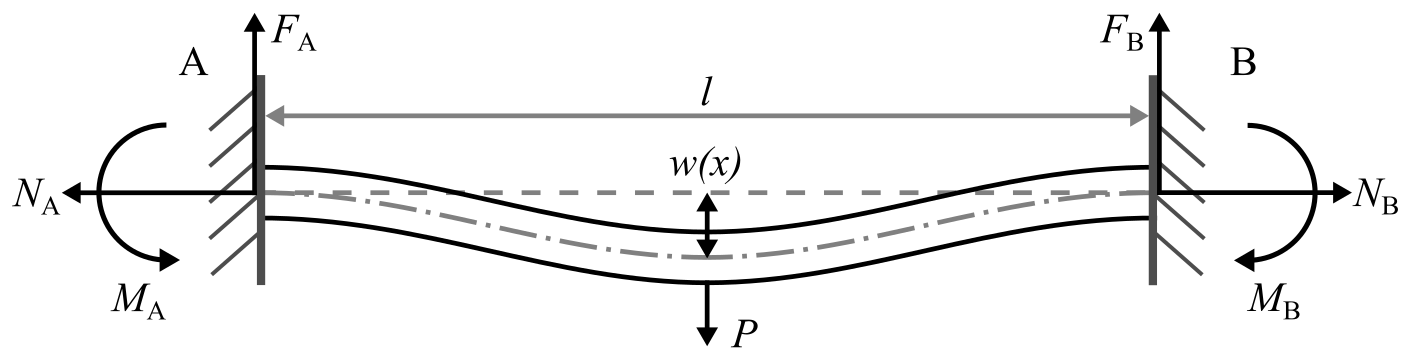
\includegraphics[width=4.7in]{Figures/FFB_Figure.png}
		\caption[FFB] 
		%>>>> use \label inside caption to get Fig. number with \ref{}
		{ \label{fig:FFB} 
			Free body diagram of a fixed-fixed beam subjected to a transverse point load.}
	\end{figure} 
	
	\textbf{Explanation for Trotter:} This is the main rule that tells us how the beam bends and moves when a force is applied.
	
	\section*{Weak Formulation}
	
	Multiplying by a test function $v(x)$ and integrating over the beam length $L$:
	\begin{equation}
		\int_0^L \left( EI w''''(x) v(x) + N w''(x) v(x) + \rho A w_{tt}(x, t) v(x) \right) dx = 0.
	\end{equation}
	Applying integration by parts twice,
	\begin{equation}
		\int_0^L EI w''(x) v''(x) dx + \int_0^L N w''(x) v(x) dx + \int_0^L \rho A w_{tt}(x, t) v(x) dx = 0.
	\end{equation}
	
	\textbf{Explanation for Trotter:} We multiply the equation by another function and integrate it. This helps us break the beam into smaller pieces for easier calculations.

	
	\section*{Finite Element Approximation}
	
	We approximate the displacement field as
	\begin{equation}
		w(x,t) = \sum_{j=1}^{N} w_j(t) \phi_j(x),
	\end{equation}
	where $\phi_j(x)$ are the shape functions.
	For an element of length $h$, the shape functions $\Phi(x)$ and corresponding nodal degrees of freedom are:
	\begin{equation}
		W_e = \begin{bmatrix} u_1 & w_1 & \theta_1 & u_2 & w_2 & \theta_2 \end{bmatrix}^{\intercal}.
	\end{equation}
	Here, \( u_1 \) and \( u_2 \) are the axial displacements at nodes 1 and 2, \( w_1 \) and \( w_2 \) are transverse displacements, and \( \theta_1 \) and \( \theta_2 \) are rotations. This ordering groups all DOFs by node and separates axial from bending behavior for clarity. Thus,
	\begin{equation}
		w_e(x, t) = \Phi(x) W_e(t).
	\end{equation}

	\begin{figure} [H]
		\centering
		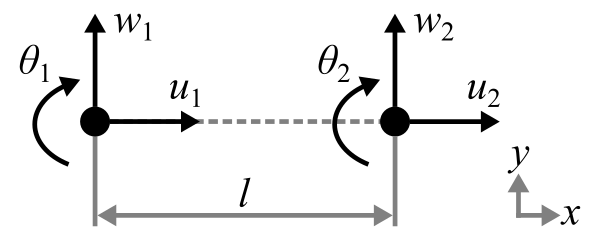
\includegraphics[width=2.0in]{Figures/1dElementDOFs_Figure.png}
		\caption[DOFs] 
		%>>>> use \label inside caption to get Fig. number with \ref{}
		{ \label{fig:DOFs}
			Degrees of freedom and internal forces for a 1D beam finite element. } 
		\end{figure} 
	
	\textbf{Explanation for Trotter:} We chop the beam into smaller sections and use math functions (shape functions) to describe how each section moves.
	
	\section*{Element Stiffness and Mass Matrices}
	
	For each beam element, a stiffness matrix and a mass matrix must be constructed. The stiffness matrix represents the resistance of the element to deformation under applied forces, accounting for both axial and bending effects. The displacement vector for each element is defined as:
	\[
	W_e = [u_1,\ w_1,\ \theta_1,\ u_2,\ w_2,\ \theta_2]^{\mathrm{T}}
	\]
	
	The element stiffness matrix is given by:
	\begin{equation}
		K_{ij}^{(e)} = \int_0^h EA\, \phi_i'(x) \phi_j'(x)\, dx + \int_0^h EI\, \psi_i''(x) \psi_j''(x)\, dx,
	\end{equation}
	where:
	\begin{itemize}
		\item \( \bm{\phi}(\xi) \) is the vector of linear Lagrange shape functions for axial displacement \( u(x) \),
		\item \( \bm{\psi}(\xi) \) is the vector of Hermite cubic shape functions for transverse displacement \( w(x) \).
	\end{itemize}
	
	Both shape functions are defined on the reference element \( \xi = x/h \in [0,1] \).
	
	The Lagrange shape functions for axial displacement are:
	\begin{equation}
		\bm{\phi}(\xi) = 
		\begin{bmatrix}
			1 - \xi \\
			\xi
		\end{bmatrix}
	\end{equation}
	
	The Hermite shape functions for transverse displacement are:
	\begin{equation}
		\bm{\psi}(\xi) =
		\begin{bmatrix}
			1 - 3\xi^2 + 2\xi^3 \\
			h(\xi - 2\xi^2 + \xi^3) \\
			3\xi^2 - 2\xi^3 \\
			h(-\xi^2 + \xi^3)
		\end{bmatrix}
	\end{equation}
	
%	These correspond respectively to \( w_1, \theta_1, w_2, \theta_2 \), and satisfy the interpolation properties:
%	\[
%	\begin{aligned}
%		\psi_1(0) = 1,\ \psi_1'(0) = 0,\quad &\psi_1(1) = 0,\ \psi_1'(1) = 0 \\
%		\psi_2(0) = 0,\ \psi_2'(0) = 1,\quad &\psi_2(1) = 0,\ \psi_2'(1) = 0 \\
%		\psi_3(0) = 0,\ \psi_3'(0) = 0,\quad &\psi_3(1) = 1,\ \psi_3'(1) = 0 \\
%		\psi_4(0) = 0,\ \psi_4'(0) = 0,\quad &\psi_4(1) = 0,\ \psi_4'(1) = 1
%	\end{aligned}
%	\]
	
	Taking the appropriate derivatives and integrating, the assembled stiffness matrix becomes:
	\begin{equation}
		K_e = 
		\frac{EA}{h}
		\begin{bmatrix}
			1 & 0 & 0 & -1 & 0 & 0 \\
			0 & 0 & 0 & 0 & 0 & 0 \\
			0 & 0 & 0 & 0 & 0 & 0 \\
			-1 & 0 & 0 & 1 & 0 & 0 \\
			0 & 0 & 0 & 0 & 0 & 0 \\
			0 & 0 & 0 & 0 & 0 & 0 \\
		\end{bmatrix}
		+
		\frac{EI}{h^3}
		\begin{bmatrix}
			0 & 0 & 0 & 0 & 0 & 0 \\
			0 & 12 & 6h & 0 & -12 & 6h \\
			0 & 6h & 4h^2 & 0 & -6h & 2h^2 \\
			0 & 0 & 0 & 0 & 0 & 0 \\
			0 & -12 & -6h & 0 & 12 & -6h \\
			0 & 6h & 2h^2 & 0 & -6h & 4h^2 \\
		\end{bmatrix}
	\end{equation}
	
	Similarly, the mass matrix accounts for the distribution of mass within the element and its contribution to the element’s dynamic behavior:
	\begin{equation}
		M_{ij}^{(e)} = \int_0^h \rho A\, \phi_i(x) \phi_j(x)\, dx + \int_0^h \rho A\, \psi_i(x) \psi_j(x)\, dx.
	\end{equation}
	
	The resulting element mass matrix is:
	\begin{equation}
		M_e =
		\frac{\rho A h}{6}
		\begin{bmatrix}
			2 & 0 & 0 & 1 & 0 & 0 \\
			0 & 0 & 0 & 0 & 0 & 0 \\
			0 & 0 & 0 & 0 & 0 & 0 \\
			1 & 0 & 0 & 2 & 0 & 0 \\
			0 & 0 & 0 & 0 & 0 & 0 \\
			0 & 0 & 0 & 0 & 0 & 0 \\
		\end{bmatrix}
		+
		\frac{\rho A h}{420}
		\begin{bmatrix}
			0 & 0 & 0 & 0 & 0 & 0 \\
			0 & 156 & 22h & 0 & 54 & -13h \\
			0 & 22h & 4h^2 & 0 & 13h & -3h^2 \\
			0 & 0 & 0 & 0 & 0 & 0 \\
			0 & 54 & 13h & 0 & 156 & -22h \\
			0 & -13h & -3h^2 & 0 & -22h & 4h^2 \\
		\end{bmatrix}
	\end{equation}
	
	\textbf{Explanation for Trotter:} We put together all the small beam sections into one big system that represents the full beam.
	
	\section*{Equation of Motion and Time Integration}
	
	The discretized equation of motion is:
	\begin{equation}
		M \ddot{W} + C \dot{W} + K W = F(t),
	\end{equation}
	where the damping matrix is given by
	\begin{equation}
		C = \alpha M + \beta K.
	\end{equation}
	Using Newmark-Beta time integration,
	\begin{equation}
		W_{n+1} = W_n + \dot{W}_n \Delta t + \frac{1}{2} \ddot{W}_n \Delta t^2,
	\end{equation}
	we solve:
	\begin{equation}
		(K + \frac{\gamma}{\beta \Delta t} C + \frac{1}{\beta \Delta t^2} M) W_{n+1} = F_{n+1} + \text{previous terms}.
	\end{equation}
	
	\textbf{Explanation for Trotter:} The beam moves over time, so we use math formulas to predict how it bends at each moment.
	
	\section*{Control Force Calculation}
	Control forces are introduced at selected nodes along the beam to actively influence both axial and bending responses. As shown in Figure~\ref{fig:control_forces}, each actuator applies a concentrated axial force \( F_{\text{control}} \) along the beam axis and induces a moment \( M_{\text{control}} \) by acting off-center relative to the beam’s neutral axis. These control actions are designed to counteract undesirable vibrations or deflections and are computed based on real-time deviations from a desired trajectory or shape.
	
	The control force is defined as
	\begin{equation}
		F_{\text{control}} = K_{\text{ctrl}} \cdot e(t),
	\end{equation}
	where \( K_{\text{ctrl}} \) represents a control gain (or gain matrix) and \( e(t) \) is the error between the measured and desired beam states. The corresponding moment is defined as
	\begin{equation}
		M_{\text{control}} = F_{\text{control}} \cdot \frac{h}{2},
	\end{equation}
	where \( h \) is the beam thickness, and the factor \( h/2 \) accounts for the distance from the neutral axis to the surface where the actuator applies the force.
	
	In the finite element framework, \( F_{\text{control}} \) is applied to the axial degree of freedom \( u \) at the control node, while \( M_{\text{control}} \) contributes to the rotational degree of freedom \( \theta \) at the same node. These contributions are inserted directly into the global force vector in the positions corresponding to those degrees of freedom.
	
	The modified equation of motion, including the control forces and moments, becomes
	\begin{equation}
		M \ddot{W} + C \dot{W} + K W = F_{\text{control}}(t),
	\end{equation}
	where \( M \), \( C \), and \( K \) are the assembled global mass, damping, and stiffness matrices, and \( F_{\text{control}}(t) \) contains the time-varying control inputs mapped to the appropriate DOFs.
	
	\begin{figure}[h!]
		\centering
		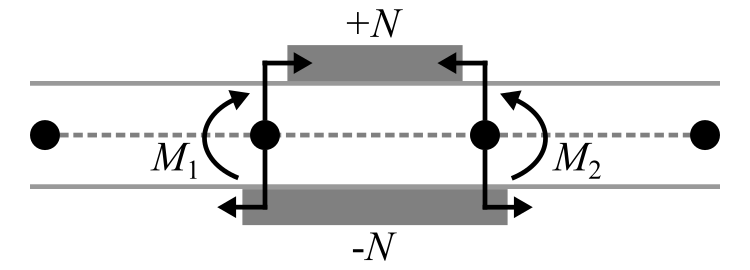
\includegraphics[width=2.4in]{Figures/ControlForces_Figure.png}
		\caption{Control force \( F_{\text{control}} \) and generated moment \( M_{\text{control}} \) applied at the control node.}
		\label{fig:control_forces}
	\end{figure}
	
	\textbf{Explanation for Trotter:} The control force is calculated based on how much the beam is off from where you want it to be (for example, how much it's bending or moving). This force is applied at a specific point on the beam, called the control node, which could be the middle or another part. The control force is an axial force, meaning it pushes or pulls along the length of the beam. Along with this, a moment (or turning force) is created by the control force, which helps control the bending of the beam. Both the pushing/pulling force and the moment are used to adjust the beam’s movement, and these changes are included in the equations that describe how the beam behaves, making sure it bends the way you want it to.

\end{document}
